\documentclass[a4paper, 11pt]{report}
\usepackage{tabularx}
%\usepackage{algorithmicx}
\usepackage{amssymb}
\usepackage{amsmath}
\usepackage{graphicx}
\usepackage{enumerate}
\usepackage{longtable}
\usepackage{array}
\usepackage[dvipsnames]{xcolor}
\usepackage[hidelinks]{hyperref}
\usepackage{xspace}
\usepackage{color}
\usepackage{tikz}
\usetikzlibrary{shapes,calc}
\usepackage{ltxcmds}

\begin{document}
	
	%%%%%%%%%%%%%%%%%%%%%%%%%%%%%%%%%%%%%%%%%%%%%%%%%%%%%%%%%%%%%%%%%%%%%%
	%% Front page
	%%%%%%%%%%%%%%%%%%%%%%%%%%%%%%%%%%%%%%%%%%%%%%%%%%%%%%%%%%%%%%%%%%%%%%
	
	\thispagestyle{empty}
	\setcounter{page}{1}
	
	
	\begin{center}
		\huge
		\textbf{Dataprojekt metoder}\\
		\small
		\textbf{10.02.22}
	\end{center}


\section*{Sørensen-Dice Coefficient (DSC)}

The Sørensen–Dice coefficient (see below for other names) is a statistic used to gaug (e.g estimate or determine the amount, level, or volume of) the similarity of two samples. \\

So if we have an image segmentation of lets say the brain created by an Deep Learning algorithm and a standard "ground truth" coming from the ATLAS segmentation, we can calculate the Dice coefficient to in a way find the similarity of the two images. The higher the coefficient, the more similarity. Anything above 0.8 is seen as almost perfect and above 0.9 perfect. \\

Simply put, the volumtetric dice Coefficient is 2 * the volume overlap divided by the total volume of pixels in both images:

$$
DSC = \frac{2(A \cap B)}{A+B}
$$
where $A$ and $B$ are volumes.\\

The DSC is used in image segmentation, especially in the medical industry. Today it is one of the most broadly used tool in the validation of image segmentation algorithms created with AI.

\section*{Hausdorff Distance (HD)}

Hausdorff distance is the "maximum distance of a set to the nearest point in the other set". given by:\\
$$
h(A, B)=\max _{a \in A}\left\{\min _{b \in B}\{d(a, b)\}\right\}
$$ where $d$ is the Euclidean distance. \\

Hausdorff distance measures how far two subsets of a metric space are from each other. Informally, it is the greatest of all distances from a point in one set to the closest point in the other set.  \\

The Hausdorff Distance is commonly used in computer vision. In that field, a typical
problem is that you are given an image and a model of what you want to match to.

\section*{Average Surface Distance (ASD)}

The average surface distance (ASD)  calculates the average of the minimum distances from every point in surface A to every
point in surface B, and vice versa, and returns the average of the two average distances. 
\\\\This tell us how much, on average, the surface varies between the segmentation and the "ground truth" (often in mm). Can be calculated as:
$$
\frac{1}{2}(h(A, B)+h(B, A))
$$
where
$$
h(A, B)=\frac{1}{A} \sum_{\alpha \in A} \min _{b \in B}\|a-b\|
$$
\section*{Added path length (APL)}
The added path length (APL) is a novel metric introduced by Vaassen et al. and is conceptually the distance that an editor's (e.g doctor) cursor travels when making corrections to an automated segmentation. Numerically it is the number of pixels in the corrected segmentation surface that are not shared in the automated segmentation surface. \\

Vaassen et al. demonstrated that the APL correlates better with the time required to correct a segmentation than do traditional, popular metrics such as the volumetric Dice similarity coefficient or the Hausdorff distance. As a measure of autosegmentation spatial similarity to a reference segmentation, the APL captures the expected time-savings benefit of automated segmentation better than traditional metrics. \\

Can be calculated as: 

$$
A-(A \cap B)
$$
where $A$ is the manually corrected segmentation surface and $B$ is the autosegmentation surface.\\

Link til noget nice kode: https://github.com/kkiser1/Autosegmentation-Spatial-Similarity-Metrics

\section*{Visualization of Methods}

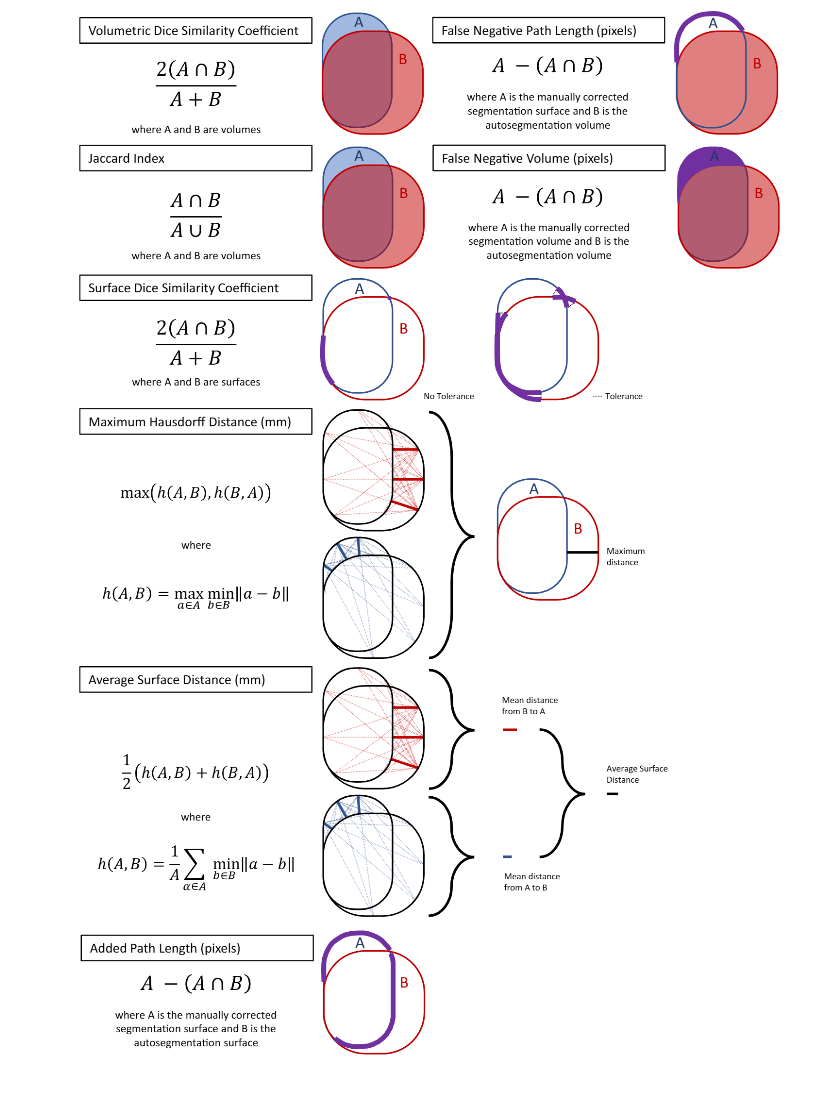
\includegraphics[width=1.0\textwidth]{methods}

\end{document}